\section{Auswertung}
\label{sec:Auswertung}

Die im Versuch aufgenommenen Daten dienen nun zur Bestimmung der Aktivierungsenergie $W$ und der charakteristischen Relaxationszeit $\tau_0$.
Die Auswertung der Messungen für beide Heizraten verlaufen analog und werden im Folgenden parallel durchgeführt.
In \autoref{fig:plot1} ist zunächst der gemessene Relaxationsstrom in Abhängigkeit von der Temperatur aufgetragen.

\begin{figure}[H]
  \begin{subfigure}{\textwidth}
  \centering
  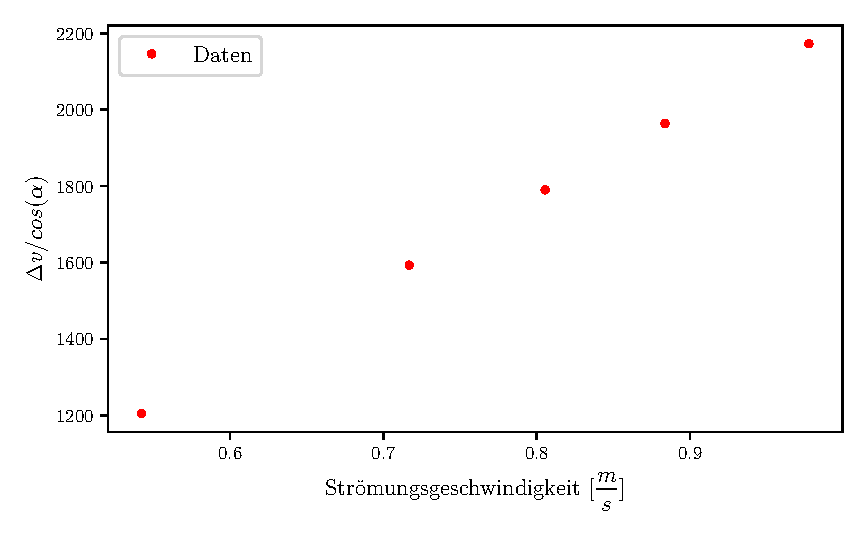
\includegraphics[width=\textwidth]{build/plot1.pdf}
  \caption{Messung 1.}
  \label{fig:plot1a}
  \end{subfigure}
  \hfill
  \begin{subfigure}{\textwidth}
  \centering
  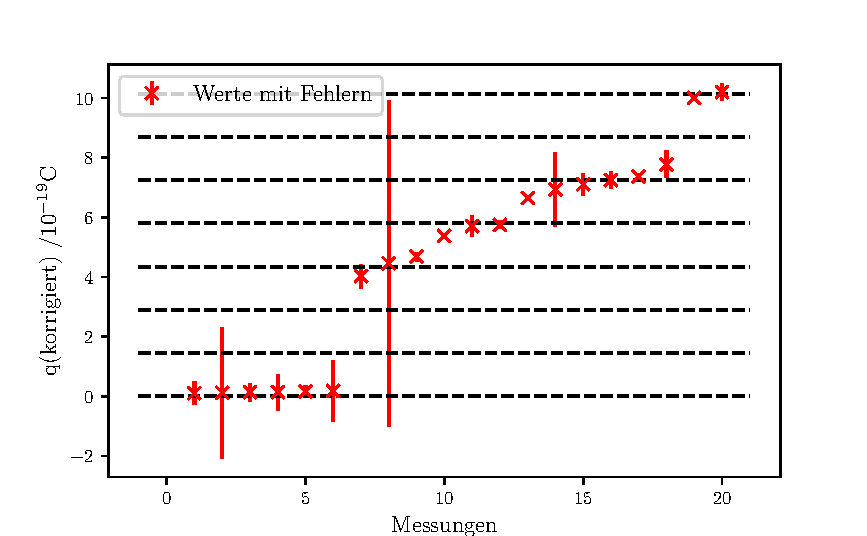
\includegraphics[width=\textwidth]{build/plot3.pdf}
  \caption{Messung 2.}
  \label{fig:plot1b}
  \end{subfigure}
  \caption{Depolarisationsstrom in Abhängigkeit von der Temperatur mit Regression für den Untergrund.}
  \label{fig:plot1}
\end{figure}

Die mittlere Heizrate berechnet sich zu
\begin{align*}
  b_1&= \qty{1.964 \pm 0.044}{\kelvin\per\minute}\\
\intertext{in Messung 1, und}
  b_2 &= \qty{1.465 \pm 0.028}{\kelvin\per\minute}\\
\intertext{in Messung 2.}
\end{align*}

Da wenige Werte im gleichen Temperaturbereich in beiden Kurven stark vom restlichen Kurvenverlauf abweichen, wird eine Regression mittels
einer Gauß-Kurve durchgeführt und die Werte entsprechend korrigiert. Im Weiteren wird nun mit den korrigierten Werten gearbeitet.
Da das erste Maximum des Relaxationsstroms, welches im Folgenden genauer
untersucht wird, auf der steigenden Flanke des zweiten Maximums liegt, wird dieser
”Untergrund” von den Messwerten abgezogen.
Das zweite Maximum entsteht durch den Dipolstrom der Wassermoleküle, welche sich bei höheren Temperaturen am Ionenkristall anlagern.
Um den Untergrund zu bestimmen wird eine Regression der Form
\begin{align*}
  f(T)= a * \text{exp}(-c/T)
\end{align*}
an den Messwerten durchgeführt die außerhalb der Maximumskurve liegen.
Der so errechnete Untergrund wird von den Messwerten abgezogen.
In \autoref{fig:plot2} sind die bereinigten Messwerte dargestellt.

\begin{figure}[H]
  \begin{subfigure}{\textwidth}
  \centering
  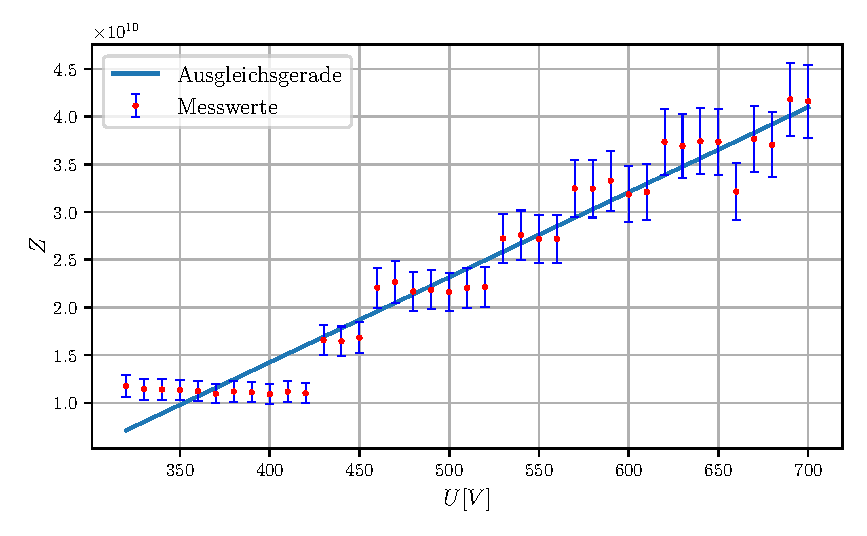
\includegraphics[width=\textwidth]{build/plot2.pdf}
  \caption{Messung 1.}
  \label{fig:plot2a}
  \end{subfigure}
  \hfill
  \begin{subfigure}{\textwidth}
  \centering
  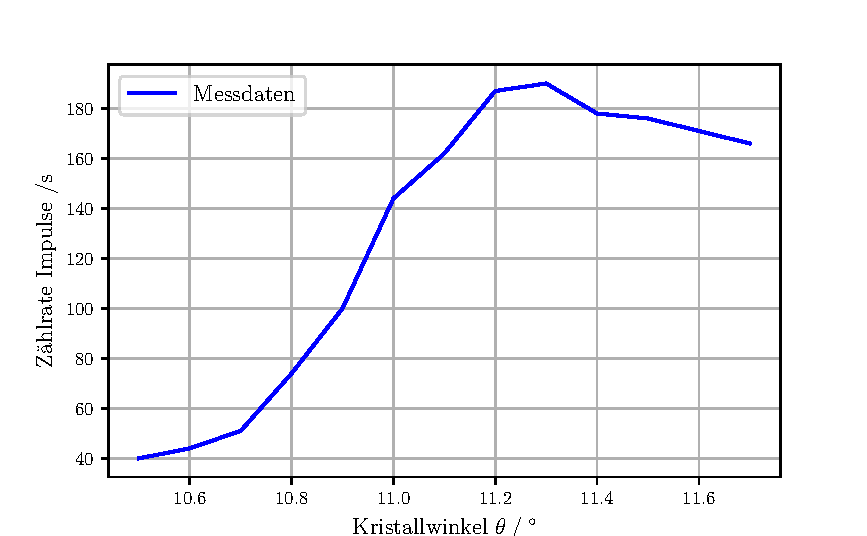
\includegraphics[width=\textwidth]{build/plot4.pdf}
  \caption{Messung 2.}
  \label{fig:plot2b}
  \end{subfigure}
  \caption{Um den Untergrund bereinigte Messwerte des Depolarisationsstroms.}
  \label{fig:plot2}
\end{figure}



\subsection{Berechnung der Aktivierungsenergie W}
\label{subsec:Aktivierungsenergie}

Die Werte die für die Bestimmung der Aktivierungsenergie $W$ mit Hilfe der Anlaufkurve des Maximums verwendet werden sind in \autoref{fig:plot2}
schwarz markiert.
Für die Bestimmung der Aktivierungsenergie unter Verwendung des gesamten Kurvenverlaufs werden sowohl die schwarz, als auch die blau
markierten Werte aus \autoref{fig:plot2} verwendet.

\subsubsection{Bestimmung mit Hilfe der Anlaufkurve des Maximums}

In \autoref{fig:plot3} werden die schwarz markierten Messwerte betrachtet. Sie werden logarithmiert gegenüber von $\frac{1}{T}$ aufgetragen
und können somit durch \autoref{eqn:kurz} genähert werden, welche logarithmisch gegen $\frac{1}{T}$ einer Gerade enstspricht.

\begin{figure}[H]
  \begin{subfigure}{\textwidth}
  \centering
  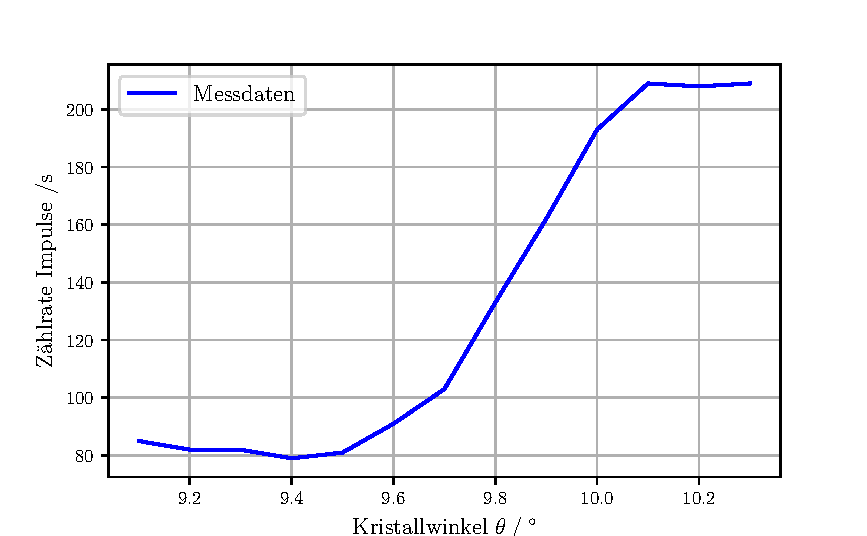
\includegraphics[width=\textwidth]{build/plot5.pdf}
  \caption{Messung 1.}
  \label{fig:plot3a}
  \end{subfigure}
  \hfill
  \begin{subfigure}{\textwidth}
  \centering
  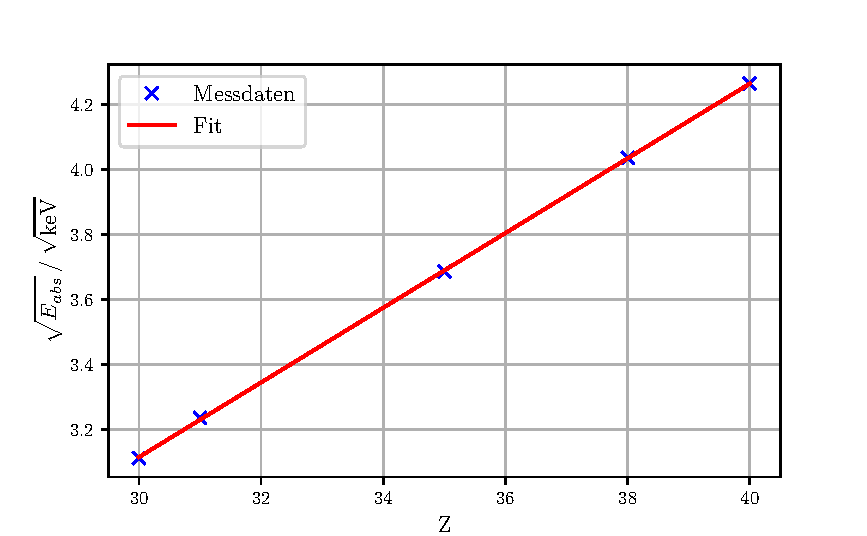
\includegraphics[width=\textwidth]{build/plot8.pdf}
  \caption{Messung 2.}
  \label{fig:plot3b}
  \end{subfigure}
  \caption{Lineare Regression der Anlaufkurve des ersten Maximums.}
  \label{fig:plot3}
\end{figure}

Die Parameter der lineraren Regressionen nach der Form
\begin{equation}
  f\Bigl(\frac{1}{T}\Bigr)= -m\cdot \frac{1}{T} +d
\end{equation}
ergeben sich zu
\begin{align*}
  m_1 &= 5831.79 \pm 677.47 \\
  m_2 &= 8727.17 \pm 497.87\\
  d_1 &= 24.54 \pm 2.83\\
  d_2 &= 37.54 \pm 2.11.\\
\end{align*}

Die Aktivierungsarbeit berechnet sich somit nach \autoref{eqn:W} zu
\begin{align*}
  W_{1,\text{Anlauf}} &= (0.50 \pm 0.06) \unit{\electronvolt}\\
  W_{2,\text{Anlauf}} &= (0.75 \pm 0.04) \unit{\electronvolt}.\\
\end{align*} 

\subsubsection{Verwendung des gesamten Kurvenverlaufs}

Um die Aktivierungsenergie $W$ über die Methode der Integration zu bestimmen, werden die Messwerte des gesamten Kurvenverlaufs des ersten 
Maximums aus \autoref{fig:plot2} verwendet.
Die Werte werden integriert und logarithmiert gegenüber $\frac{1}{T}$ aufgetragen und können durch \autoref{eqn:int} analog zum vorherigen
Abschnitt zu einer Gerade angenähert werden.
Sowohl die integrierten Werte, als auch die Regressionsgerade sind in \autoref{fig:plot4} dargestellt.

\begin{figure}[H]
  \begin{subfigure}{\textwidth}
  \centering
  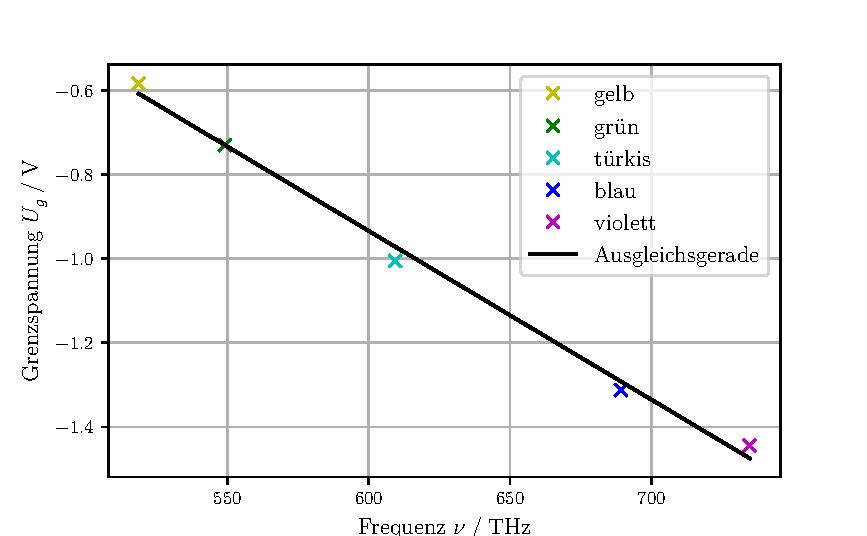
\includegraphics[width=\textwidth]{build/plot7.pdf}
  \caption{Messung 1.}
  \label{fig:plot4a}
  \end{subfigure}
  \hfill
  \begin{subfigure}{\textwidth}
  \centering
  \includegraphics[width=\textwidth]{build/plot10.pdf}
  \caption{Messung 2.}
  \label{fig:plot4b}
  \end{subfigure}
  \caption{Lineare Regression der integrierten Kurven.}
  \label{fig:plot4}
\end{figure}

Die Ausgleichsrechnung ergibt die Parameter
\begin{align*}
  e_1 &= 5422.63 \pm 418.39 \\
  e_2 &= 5935.77 \pm 531.90 \\
  f_1 &= 24.53 \pm 1.70 \\
  f_2 &= 26.64 \pm 2.17. \\
\end{align*}

Daraus bestimmt sich die Aktivierungsenergie zu 
\begin{align*}
  W_{1,\text{Integral}} &= (0.47 \pm 0.04) \unit{\electronvolt}\\
  W_{2,\text{Integral}} &= (0.51 \pm 0.04)\unit{\electronvolt}.\\
\end{align*} 


\subsection{Berechnung der charakteristischen Relaxationszeit}

Um die Relaxationszeit zu berechnen werden zunächst aus \autoref{fig:plot2} die Temperaturen $T_\text{max}$ bestimmt, an denen $I$ maximal ist.
Diese enstsprechen
\begin{align*}
  T_\text{max1} &= \qty{259.45}{\celsius}\\
  T_\text{max2} &= \qty{249.55}{\celsius}.\\
\end{align*}

Durch Einsetzen der Maximaltemperaturen, sowie der in den vorherigen Abschnitten bestimmten Aktivierungsenergien
in \autoref{eqn:taumaxsource} ergeben sich die charakteristischen Relaxationszeiten zu
\begin{align*}
  \tau_{01,\text{Anlauf}} &= \qty{1.26 (15)e-18}{\second}\\ 
  \tau_{01,\text{Integral}} &=\qty{1.36 (11)e-18}{\second}\\
  \tau_{02,\text{Anlauf}} &= \qty{7.80 (50)e-19}{\second}\\
  \tau_{02,\text{Integral}} &=\qty{1.15 (0.10)e-18}{\second}.\\
\end{align*}
